\section{Reconstructing the exploration and pilot decisions}
\label{sec:results}

\subsection{Calibration coverage and reasons for rejection}

Our secondary analysis script rebuilds all 76 configuration-by-seed loss
contrasts for the \RoneCells-cell exploration directly from archived
metrics before verifying the published cell and seed summaries
(\artifact{R1}). Pilot reconciliation follows a parallel path. Across 66
run-metrics files and 126 saved candidate-probe records, the script
recomputes paired utility and gain differences, null-adjusted property and
structure probe advantages, and composite eligibility flags against the
archived verification report (\artifact{P4}). All checks operate strictly
on saved numerical outputs, and Table~\ref{tab:cohorts} summarises the
resulting experimental units and failure counts.

\begin{table}[t]
\centering\small
\begin{tabularx}{\linewidth}{@{}lXX@{}}
\toprule
 & Exploration & Defence-redesign pilot \\
\midrule
Candidate configurations & \RoneCells & \PfourCells \\
Repetitions per candidate & 4 training seeds & 3 paired seeds \\
Recorded scope & Frozen exploratory rules & Frozen exploratory pilot \\
Qualified breach or failed composite & \RoneQualifiedBreaches & \PfourPrivacyFailures \\
Privacy undetermined & \RoneUndetermined & \PfourPrivacyUndetermined \\
Utility failures & \RoneUtilityFailures & \PfourUtilityFailures \\
Gain failures & \RoneGainFailures & 0 \\
Eligible candidate & None & None \\
\bottomrule
\end{tabularx}
\caption{Configuration counts and gate outcomes across both multi-cell
campaigns. Rejection causes in the \RoneCells-cell exploration overlap,
whereas the seven-cell pilot applies an all-bindings composite privacy
policy across its candidate mechanisms (\artifact{R1}, \artifact{P4}).}
\label{tab:cohorts}
\end{table}

Qualified privacy breaches eliminate \RoneQualifiedBreaches\ candidates
outright. Independent utility or remote-gain failures account for the
remaining \RoneUndetermined\ configurations and leave zero viable splits
under the frozen exploratory rules. Even if all 20 unqualified probes were
rebuilt and passed calibration, newly qualified measurements could only add
further breach flags without overturning any recorded rejection.

Uncertainty estimators also differ structurally between the two campaigns.
Exploratory cells apply two-sided 95\% Student-$t$ intervals over four
independent seeds, whereas pilot utility gates enforce a one-sided 95\%
upper Student-$t$ bound ($t_{0.95,2}=2.919986$) across three paired seeds.
Both conventions remain distinct throughout our reanalysis scripts.
Disjoint combinations of rejection causes appear separately in
Table~\ref{tab:intersections} (Appendix~\ref{app:checks}) so readers can
inspect exact failure overlaps without conflating heterogeneous confidence
rules.

Separating atomic probe readouts from composite campaign labels clarifies
what happened inside the defence pilot. Atomic leakage stays visible. Every
pilot cell recorded calibrated next-byte structure breaches ($0.097$ to
$0.112$, with all 21 of 21 seed bindings qualified) and qualified
punctuation-property advantages ($0.79$ to $0.89$), yet when one or two
seed bindings for the punctuation-property probe stepped outside the
$\pm 0.02$ null band, the all-bindings rule labelled the composite cell
undetermined even though concrete calibrated leakage was already measured.
Figure~\ref{fig:campaigns} displays gate outcomes for both multi-cell
campaigns side by side without collapsing their distinct reporting rules.

\begin{figure}[t]
\centering
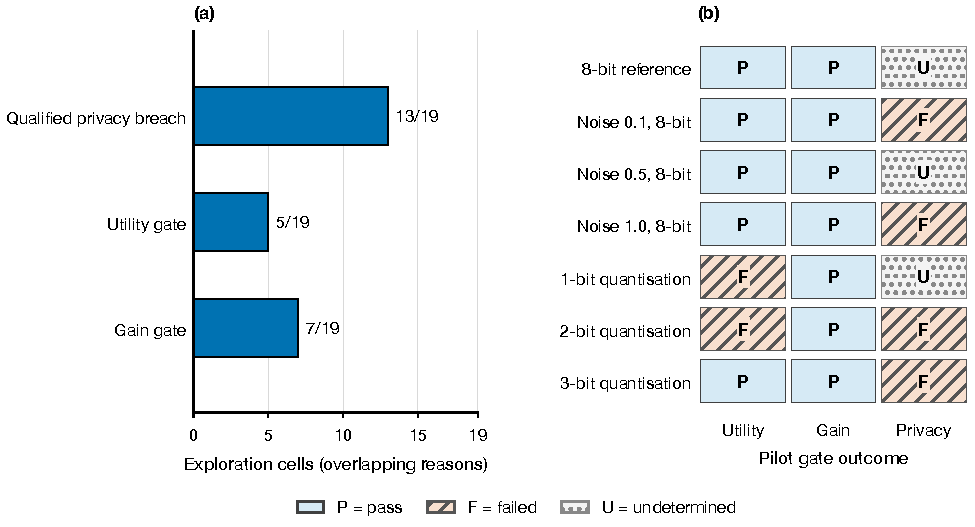
\includegraphics[width=\linewidth]{figs/campaign-gates.pdf}
\caption{Gate outcomes for the \RoneCells-cell exploration and seven-cell
defence pilot. Overlapping bars in panel~(a) tally qualified breaches,
utility losses, and gain deficits across four-seed exploratory candidates
(\artifact{R1}), while panel~(b) decomposes three-seed paired pilot cells
across utility, gain, and composite privacy rules (\artifact{P4}).}
\label{fig:campaigns}
\end{figure}

\subsection{The narrow utility margin still passes}

Exploratory utility gating requires both a four-seed mean cross-entropy
increase of at most $0.10$ nats relative to baseline and an upper 95\%
Student-$t$ confidence bound of at most $0.12$ nats. Four training seeds
yield the descriptive interval
\begin{equation}
 \bar u\;\pm\;t_{0.975,3}\,\frac{s_u}{\sqrt{4}},
 \qquad t_{0.975,3}\approx3.182446.
 \label{eq:interval}
\end{equation}
Fixed evaluation panels define the underlying loss surface across all
configurations without multiplicity correction. Figure~\ref{fig:utility}
plots both acceptance cutoffs side by side.

\begin{figure}[t]
\centering
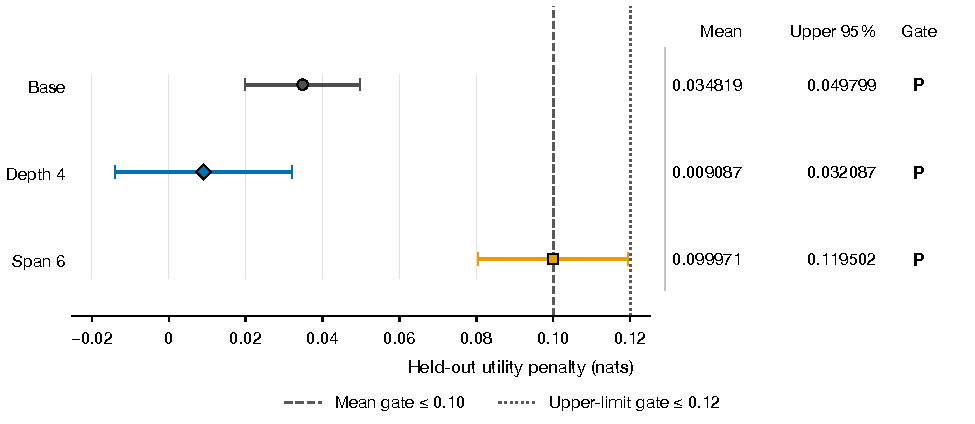
\includegraphics[width=\linewidth]{figs/r1-utility-boundary.pdf}
\caption{Utility loss deltas and descriptive two-sided 95\% Student-$t$
intervals from Eq.~\eqref{eq:interval} across four training seeds on fixed
evaluation text (\artifact{R1}). Separate vertical lines mark the
$0.10$-nat mean cutoff and the $0.12$-nat upper-endpoint cutoff, which
explains why \texttt{span-6} clears both utility criteria even though its
upper interval crosses $0.10$.}
\label{fig:utility}
\end{figure}

Configuration \texttt{span-6} illustrates how dual-statistic rules behave
near a boundary (\artifact{R1}). Across its four seeds, \texttt{span-6}
attains a mean loss increase of $0.0999705344$ nats ($2.9466\times10^{-5}$
nats below the $0.10$ cap) and an upper confidence endpoint of
$0.1195024415$ nats ($4.9756\times10^{-4}$ nats below the $0.12$ limit).
Both utility requirements pass. Archived logs reject \texttt{span-6} solely
for failing remote-learning gain and triggering a qualified privacy breach,
while \texttt{depth-4} posts a smaller four-seed mean loss delta than the
base split within this exploratory cohort.
